\documentclass{article}
\usepackage[utf8]{inputenc}
\usepackage[a4paper, width=160mm, top=20mm, bottom 20mm]{geometry}
\usepackage{graphicx}
\usepackage{float}
\usepackage{ulem}
\usepackage{forest}
\usepackage{tikz}
\usetikzlibrary{positioning}

\newcommand{\wrap}[1]{\parbox{1\linewidth}{\vspace{1.5mm}#1\vspace{1mm}}}

\setlength{\textheight}{25.7cm}
\setlength{\textwidth}{16cm}
\setlength{\unitlength}{1mm}
\setlength{\topskip}{2.5truecm}
\topmargin 260mm \advance \topmargin -\textheight 
\divide \topmargin by 2 \advance \topmargin -1in 
\headheight 0pt \headsep 0pt \leftmargin 210mm \advance
\leftmargin -\textwidth 
\divide \leftmargin by 2 \advance \leftmargin -1in 
\oddsidemargin \leftmargin \evensidemargin \leftmargin
\parindent=0pt

\frenchspacing

\usepackage{microtype}
\usepackage[english]{babel}
\usepackage{listings}
\newcommand{\mylanguage}{english}


\title{Design Document}
\author{Beatrice-Andreea Vizuroiu, Cody Boon, Elena Martellucci, Kalle Struik, Mehmet Alp Sozuduz }
\date{March 2021}

\usepackage{natbib}

\begin{document}

\maketitle

\section{Responsible CS}
"In what way would our design process and final product change if we also had to design our product for one additional value of a 'non-obvious' stakeholder?" That is the question that we have to ask ourselves when creating a product.\\
\\We start by defining eight stakeholders\\
\begin{center}
    \begin{tabular}{ | l | l | l | l | l |}
    \hline
    Direct    & Indirect \\ \hline \hline
    Client  & Anyone else on the same bandwidth/with the same API  \\ \hline
    Lecturer  &??  \\ \hline
    TA  &??  \\ \hline
    Students  &   \\ \hline
    Tu Delft  &   \\ \hline
    \end{tabular}
\end{center}

\\The chosen stakeholder in which we will focus on is the \textbf{TU Delft} institution.
This is because all the users and systems have to follow its rules and regulation.\\

\\ A list of three ethical values that we presume important to TU Delft, in the context of an online system that students can ask questions on, are listed below.
\begin{itemize}
    \item Privacy:  As stated in the Student charter 2020-2021 "Your personal data can only be accessed by TU Delft staff who are directly or indirectly involved with student administration."\citep{TUDelftMan} TU Delft also outlines a number of legal rights, such as: right of inspection, right to rectification and supplementation, right to object, right to data portability, right to be forgotten, right to restriction of processing and right to file a complaint.
    Therefore as a product designed to be used within the TU Delft ecosystem we need to assure that it follows the whole protocol.
    \item House rules and disciplinary measures: Specifically regarding the use of Educational ICT Facilities, there are some rules that students have to follow when using it.
    Examples are using a falsified identity, use for educational purposes and  the violation of copyright and intellectual property rights.
    This is important because a large number of students may be using these facilities when using the program, therefore the program has to adhere to these regulations.\citep{TUDelftICT} (maybe change this one because it is not related to anything we will be doing, i.e.in person stuff)
    \item Code of Ethics: All members of the TU Delft have to follow a Code of Ethics, which includes but is not limited to what to do if you see behaviour that you consider to be inappropriate or (in more serious cases) what to do if you see someone breaking any of the rules stated above.\citep{TUDelftMan}
\end{itemize}

\\ To find a definition of privacy in the context of a forum in which students can ask questions, it is first important to understand the difference between \textbf{the right of privacy} and \textbf{private information}.
The right of privacy is a legal definition that requires the ability to keep personal life secret if the person wishes so, this encompasses  personal information/activities/spaces. Therefore the information privacy is a subsection of the right of privacy, which in the context of a forum means that users have personal information that they don't want to be shared outside the approved community.\citep{PrivacyComputing}\\

\\A good example that closely relates to what we are doing are online forums.
More specifically an online tool which is very similar to our product is Pigeonhole Live (add source)  (ADD: Based on your experiences in the previous steps, an indication of what you would integrate in your design process to learn more about the chosen value and/or stakeholder, e.g., which academic literature, artworks, experts in domain different than yours etc. you would have to consult/include in your project; give some general indication: e.g. "I would discuss with social scientists who have study the phenomenon X, I would check documentaries on discrimination of the group Y, I would study legal/philosophical literature on the right to Z, political studies on the meaning of democracy etc.))\\

\\The following figure is the Values Hierarchy of the chosen ethical value (i.e.Privacy) \\

\begin{figure}[h]
    \centering
    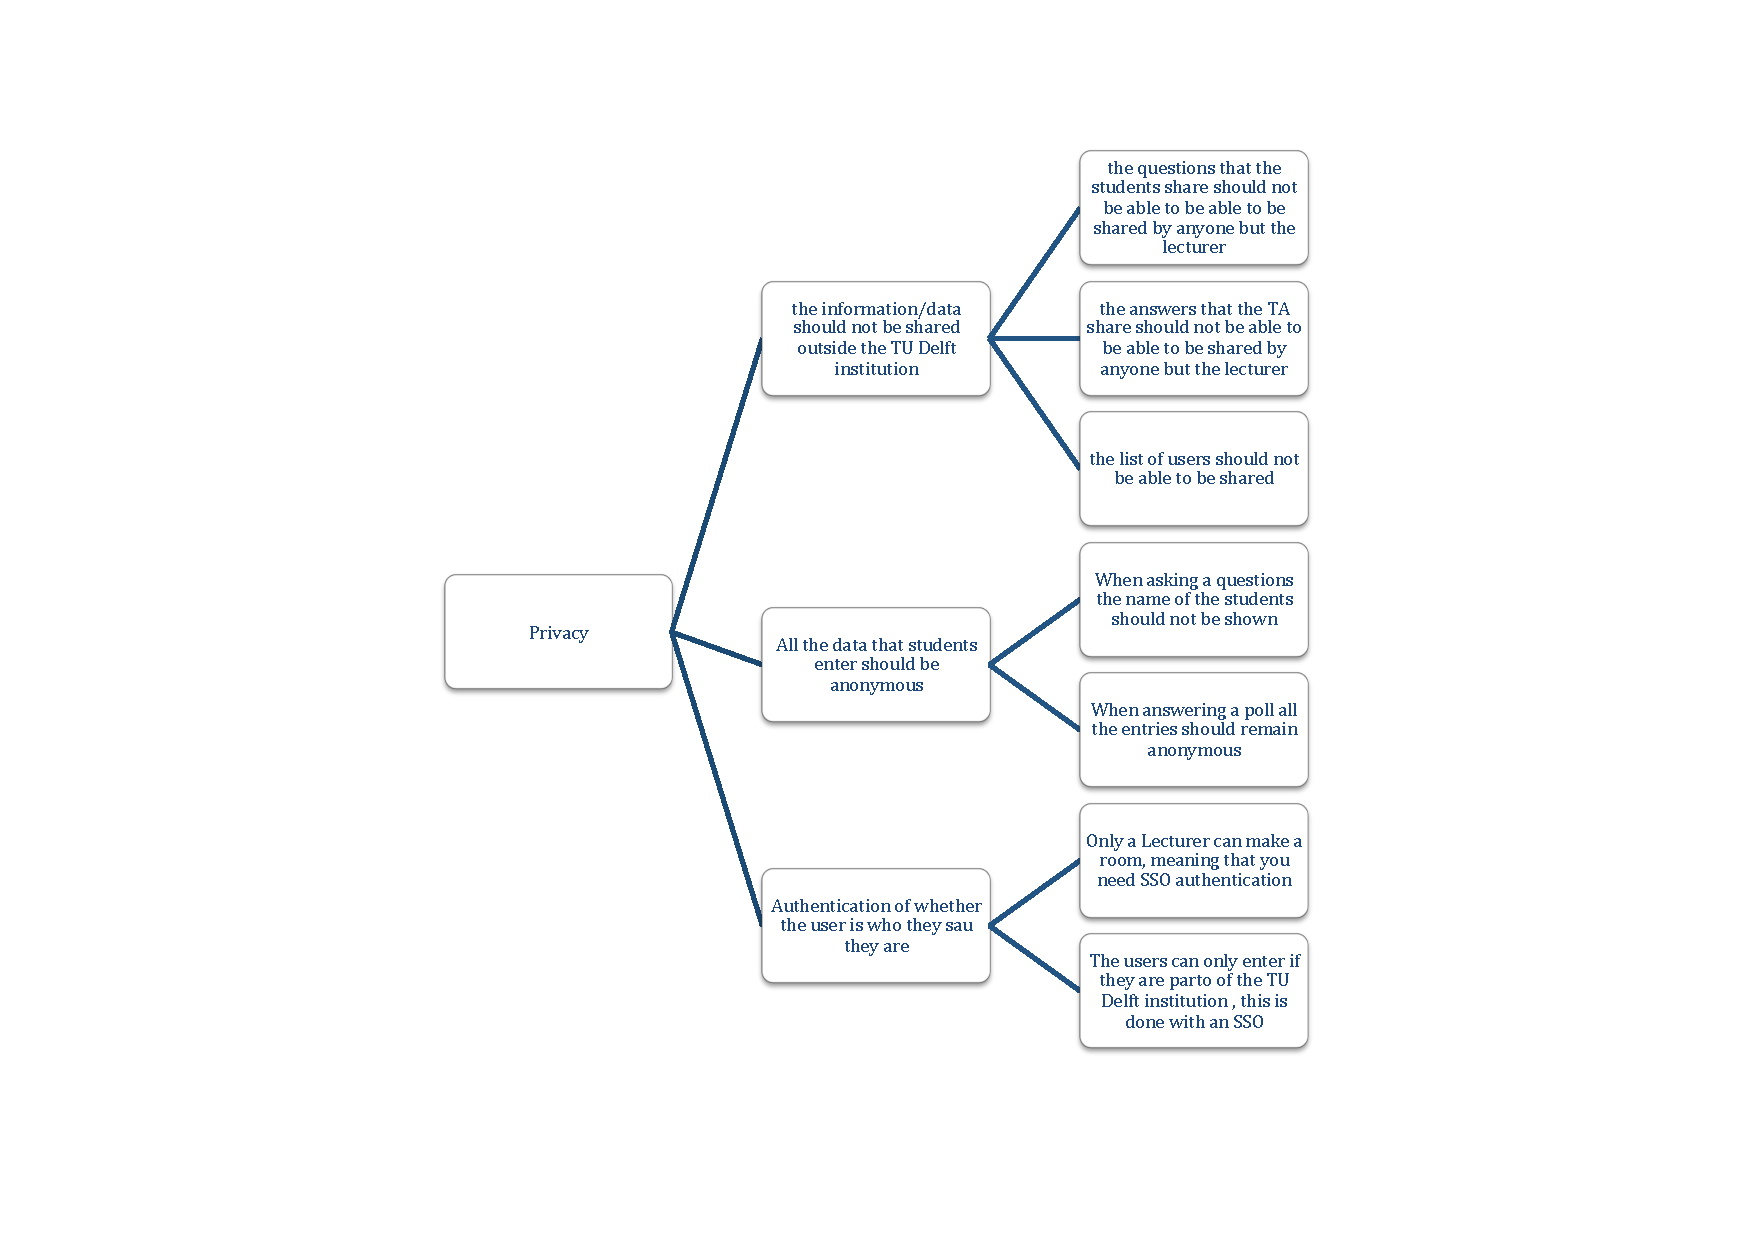
\includegraphics[width=0.9\textwidth]{Responsible_CS_tree.pdf}
    \caption{Values Hierarchy showing from left to right the value (i.e. privacy), norms and design requirements..}
    \label{fig:tree}
\end{figure}


\\The design changes that are required to account for the additional value/stakeholder will create issues, specifically regarding \textbf{authentication}.
This is because the client (stakeholder 1) and the TU Delft (stakeholder 4) want two different things.
The client specified that authentication is a "won't have" due to the difficulty working with bureaucracy and not having enough resources to implement it.
Moreover, the biggest problem is with time, simply put there isn't enough of it to work on something as important as authentication.
In contrast, TU Delft prioritises privacy, therefore not having proper authentication will cause problems in the long run.
Specifically if we want to implement the program within the TU Delft ecosystem.
This issue will be resolved if we are tasked to continue working on it, but in the current time frame authentication will not be possible to implement. \\


\section{HCI}
The objective of this Human Computer Interaction evaluation is to better understand our strengths and weaknesses in the design of our product.
As of the 14\textsuperscript{th} March we have designed a UI that encompasses all the different types of users and what they will see.
We also designed an entry page, so that all the different users can be sent to their appropriate views.\\

\subsection{Methods}
\subsubsection{Experts}
Currently, the experts that evaluate our application are made up of 5 students (from group 6) that all have around half-year experience each.
It can be argued that these "experts" should actually be considered novices, nevertheless all these students are working on the same project with the same requirements.
Therefore they should be very well informed on this specific product and its' requirements.
From now on we will refer to them as CS students.\\

\subsubsection{Procedure}
To begin, we instructed the experts on what to do by giving them the following instructions:
\begin{itemize}
    \item Download the Heuristics Evaluation document.
    \item Review the views on the Figma platform.
    \item Grade the questionnaire at the bottom of the document from 1 - 10.
    \item For any additional notes (can't find button etc.), you can simply note them down.
\end{itemize}
When referring to the Figma in the instructions, it refers the evaluators to our design on a platform called Figma.
Figma is a graphics editor, wherein the designers can link different frames together to emulate what happens when a user clicks on a a certain button.
This allows the evaluators, to get a complete experience of what the product should do.
This allows us, as designers, to see if there is a problem within the actual design, before coding it.\\

It is important to note that the contents of the Heuristics Evaluation document include the heuristics, the steps to follow and the questionnaire.\\

The heuristics which the experts should take into account while analyzing the design are:
\begin{itemize}
    \item Match between system and the real world
    \item Aesthetic and minimalist design
    \item Consistency and standards
    \item User control and freedom
    \item Visibility of system status
    \item Error prevention
    \item Recognition rather than recall
    \item Flexibility and efficiency of use
    \item Help users recognize, diagnose, and recover from errors
    \item Help and documentation
\end{itemize}
The evaluators were given the following steps to help them navigate the system:
\begin{enumerate}
    \item As a student, try to up-vote a question.
    \item As a student, try to ask a question.
    \item As a student, try to tell the lecturer if he/she is too slow/fast.
    \item As a student, try to leave a room.
    \item As a student, try to sort the questions by.
    \item As a lecturer, try to create a room.
    \item As a lecturer, try to export the questions.
    \item As a lecturer, try to mark a question as answered.
    \item As a TA, try to answer a question.
    \item As a TA, try to ban a student from the room.
    \item As a TA, try to create a poll.
\end{enumerate}
\subsection{Measures (data collection)}
After performing all the tasks the evaluators are asked to answer the following questions by giving an answer ranging from 1 to 10 (1 being very bad and 10 being very good):
\begin{enumerate}
    \item How clear is the system status?
    \item how consistent is the design of the application?
    \item how aesthetic yet simplistic is the design of the application?
    \item how easy is it to explore the functionalities of the application?
    \item how easy is it to recognize the functionality of every button?
    \item how efficient is the application?
    \item how easy is it to commit errors (ex. clicking the wrong button)?
    \item how easy is it to recognize and recover from an error (ex. clicking the wrong button)?
    \item how much help does the user receive to understand all the functionalities?
    \item how much do you see yourself using this application?
\end{enumerate}
At the end of the questionnaire they were encouraged to add any comments or suggestions that could help us, designers, improve our application design.\\

All of this has been sent in the Heuristics Evaluation document, and when the experts have finished it they send it back to us, designers.
We chose this format because it would be easier for the experts to add any comments throughout the questionnaire if they wish to do so.\\

\subsection{Results}
The following table report the results given by the 5 experts.
\begin{center}
    \begin{tabular}{|c|c|p{0.7\linewidth}|}
        \hline
        Question & Result (average) & Comments \\ \hline
        1 & 5.4 & \wrap{- Not a lot of feedback on the system status \\ - Add a green dot anywhere or something similar to indicate a connection. \\ - No status bar but can see if the system is functioning } \\ \hline
        2 & 9.0 & \wrap{- A question that I hadn’t yet up-voted was already purple \\ - System is very consistent overall and in the main design there are no differences between screens \\ - The font and size of the button/text/... vary between screens and I had to zoom/de-zoom to properly see
        everything.} \\ \hline
        3 & 7.6 & \wrap{-Lot of icons that make it less simplistic \\ - It’s pretty simple but sometimes there is a lot going on in the options bar\\ - Improve the sizing and distribution of the top right buttons \\ - A lot of icons sometimes in the right corner above makes it a little more complicated } \\ \hline
        4 & 6.0 & \wrap {- It’s hard to explore because there are no back buttons. \\ - It is mainly clear how everything works, since there is only one sub menu and there is a big question mark if you want to know what everything does \\ - I couldn’t always find the features mentioned in this document. (sorting the questions, leaving the room and answer a question) } \\ \hline
        5 & 9.2 & \wrap{- All of the symbols are common symbols so you know what to expect. Except the “export question” symbol. \\ - Except for maybe the upvote button, which could be unclear for someone not familiar, everything is quite easy to recognize. There are labels everywhere and where there are no labels, there is no need.} \\ \hline
        6 & 8 & \wrap{- Most buttons are available with very few clicks. \\ - It is  not possible to schedule a lecture  \\ - Sometimes close functions such as timeout and ban, for example only after clicking on something else since banning doesn’t happen too often} \\ \hline
        7 & 5 & \wrap {- Easy to commit errors and there is no “back” button. You could also make a different colour for text fields and buttons, that way it’s more clear.\\ - It is extremely easy to commit to an error since there is no prompt when for example deleting a question.} \\ \hline
        8 & 4.4 & \wrap {- No real error messages or back button to get out of a certain situation \\ - Not very easy to find an exit/back button \\ - There is not really a possibility to see what you have done and no return button, so to recover from an error is not possible. } \\ \hline
        9 & 7.6 & \wrap { \\ - There is a question mark but it’s not really clear what happens if you click on this \\ - I am not sure how good the help button is, but I would think that gives all the help someone may need}\\ \hline
        10 & 8.6 &  \\ \hline
    \end{tabular}
\end{center}

Note that the results show the average of the raw data.
The raw data is taken from 5 experts, therefore it is calculated using the following equation:
\[ \frac{(r_1 + r_2 + r_3 + r_4 + r_5)}{5} = average \]
Where r is the result and the number below indicates which user it is from 1 to 5.
\\

Along with the results we were given comments for each question (see table) and also general comments.
It is important to note that the table mostly includes the comments in which tips are given and not the ones that say, for example, "good simplistic design".
This is because the tips are constructive feedback that help us find what we should specifically fix.
The general comments are:
\begin{itemize}
    \item In general, it's a nice, intuitive design. However, it was hard to tell how to join as a moderator or student. It would be useful to make this more clear.
    \item It looks good. The link in the moderator view (I think?) is not functioning clearly, I couldn't tell what it does, and it is not very clear how the feedback works. For example, can a user click as many times as they want or do you stay on too slow or too fast (is it continuous feedback?), if so maybe there could be an option for not too slow or too fast, but just right.
    \item It looks really good already, maybe make it more clear when you're in a student or moderator view, I couldn't tell. I also didn't completely understand the difference between the faster and slower buttons as opposed to the circles with too fast too slow but maybe that's just the student and moderator view. (Lecturer / student difference) Maybe somewhere provide information on what it means to timeout a user (e.g. how long does this last?). Other than that nice job!
    \item Overall, it's a pretty amazing application, you have used features such as hovering, highlighting the correct features, dark mode, .... which are quiet advanced and it really looks like a professional app! Here are some remark I had when testing the app.
    \begin{itemize}
        \item When sending a question, the icon for the light/dark mode change position.
        \item When creating a new "room" the user is asked to enter the name of the lecturer, I don't think this is really necessary if the students are also allowed to create room (the course id is sufficient I think, people good start messing around with the lecturer's name and this could become offensive).
        \item You did not include anything about the time/date of the lecture, are you planning on doing so?
    \end{itemize}
\end{itemize}
As you can see, the three questions wherein we have the lowest results are (going from lowest) are question 8, 5 and 1.
The reason why and how we are going to improve it will be discussed in the Conclusion and Improvements.


\subsection{Conclusions and Improvements}
To conclude, these results show that the overall design of the application is very good with few problems here and there (specifically regarding the how recognizable buttons are(i.e. question 5)).There also seems to be notable problems regarding error notification and the status of the system (question 8 and 1 respectively).\\

Advice regarding these two problems, that were given by the experts, include:
\begin{itemize}
    \item Adding error messages to the UI.
    \item Including back buttons to be able to recover from an error or unwanted action
    \item Including a confirmation pop-up when doing something permanent (e.g. a student deleting a question)
    \item Giving feedback that denotes system status. I.e. green light to show the system is functioning correctly.
\end{itemize}

Those were a few tips from experts on how we could improve our lowest scoring points.\\

The main problems with our design are omitting necessary information, lack of confirmation/notification when performing permanent actions, and absence of "back" buttons that allow recovery from errors or unwanted actions.
To account for the first problem, we could introduce an indicator signal that will show the system status.
Another way of showing this information could be through adding explicit messages when something (error/crash) happens.
For the second problem, introducing check-boxes for users to direct their attention to the action they are performing could solve this issue.
Although the experts have stated that pop-ups would be a good alternative, we believe that these do not align with the intention of our app - a side application that lecturers and students will use to communicate their questions and answers.
For the last point, simply adding "back" buttons as recommended should solve this issue.
There are a few more less urgent remarks, such as the fact that some buttons are less recognizable than others.
If time allows it, we are planning on discussing and changing them.\\

Overall, the heuristics data shows that our overall design is minimalist and consistent.
It was, generally, received well by the experts that we contacted.
They have given us a few points to work on and improve.
We hope that through this heuristic evaluation, our app will become easier to understand and use. \\

(ADD: The conclusion of this section should show your final GUI design.)
\begin{itemize}
    \item Note that this report is only about the design, so it is not necessary to always also implement all the improvements in your real application. Do note down explicitly what you have only designed, and what you have also implemented.
\end{itemize}


\bibliographystyle{plain}
\bibliography{references}
\end{document}
